   Intel’s \gls{rapl} is a tool to measure the energy on \gls{cpu} and primary storage (\gls{dram}). Here it will explain how it got introduce, how it works, and the limitations it has.
	
	\gls{rapl} is a well-known and accepted interface for measuring the power consumption of a computer system. Various studies used this interface as a measuring tool, and others review Intel \gls{rapl} measurements in terms of accuracy, performance, granularity, usability ~\cite{raplpref,raplpref2}.
	

	Intel introduced \gls{rapl} on they compilers in the architecture of the Intel Sandy Bridge, and since the first appearance, it has been evolving in the newer architectures. \gls{rapl} has \gls{msr} that aren't part of the architecture of the processor but address power values required for energy consumption management ~\cite{raplpref,intel64and,portela2016}.
	
	
    The mains functionalities of the \gls{rapl} are to measuring the energy consumption on the \gls{cpu} and primary storage and also to limit the energy consumption on the components mentions. In the context of this research, we won't use the last functionality, as it does not fit in the context of this study ~\cite{raplpref,raplpref2,intel64and}.
	
	
	The \gls{rapl} does not measurements energy based on an analog energy meter because energy consumption is estimated through the analysis of various hardware performance counters, temperature sensors, leakage energy, and IO models.  Registers reserved for energy readings are updated approximately every millisecond (1kHz) ~\cite{energypapi,portela2016}.

    \begin{figure}[ht!]
    \centering
    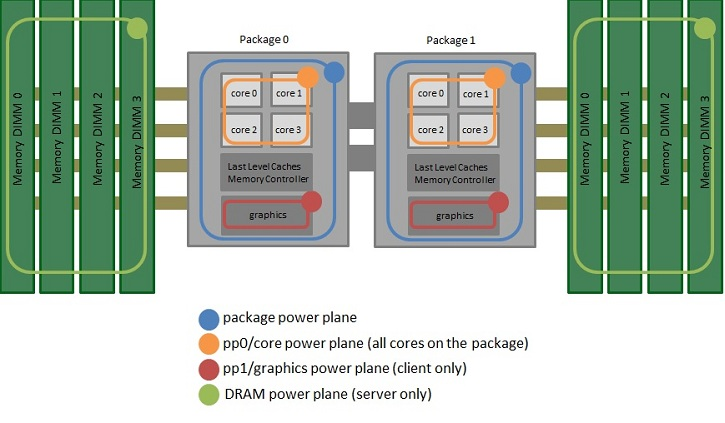
\includegraphics[width=\linewidth]{Chapters/images/power_domains2.jpg}  \caption{Intel’s \gls{rapl} Power Domain.}
    \label{fig:powerdomain}
    \end{figure}
    
    We can check the different power domains supported by \gls{rapl} in figure \ref{fig:powerdomain}. Each power domain has a different  \gls{msr}  and reports the domain's energy consumption, allowing us to limit that domain's power usage over a specified time. Each domain represents distinct physical component sets, currently, these are: 
    
    \begin{itemize}
        \item \textbf{Package}: the package domain refers to the package's energy consumption of the entire socket, including the core and uncore components energy ~\cite{intel64and}.
        \item \textbf{PP0/Core Power Plane 0}: This domain measurement the energy consumption of all processors socket~\cite{intel64and,portela2016}.
            \item \textbf{PP1/Graphics Power Plane 1}: This domain measures the energy consumed by all processors in a \gls{gpu}.
        \item \textbf{DRAM}: This Domain refers to the energy consumption of random access memory (RAM)~\cite{intel64and,portela2016}.
        \item \textbf{Psys}: Intel \textit{Skylake} has introduced a new \gls{rapl} Domain named PSys. It monitors and controls the thermal and power specifications of the entire SoC and it is particularly useful when the source of power consumption is neither the \gls{cpu} nor the \gls{gpu} \cite{raplpref}.
    \end{itemize}
    For multi-socket server systems, each socket reports its own \gls{rapl} values \cite{raplpref}.
    
    There are some distinctions between the list of available domains, depending on the type of platform. The available domains on platforms intended for the client are Package, Power Plane (PP) 0, and PP1. On the other hand, the Package, PP0, and \gls{dram} domains are available on the Platform intended for Servers \cite{raplpref2}.
    In the Table \ref{tab:rapltable} presents an overview of \gls{rapl} domains supported by different processor model.
% Please add the following required packages to your document preamble:
% \usepackage{multirow}
\begin{table}[H]
\centering
\caption{RAPL power domains supported by different models}
\begin{tabular}{|c|c|c|c|c|c|}
\hline
\multirow{ }{Model }{} & \multicolumn{5}{c|}{Power domain supported} \\ \cline{2-6} 
                       & PKG    & PPO    & PP1    & DRAM    & PSYs   \\ \hline
Sandy Bridge           & YES    & YES    & YES    & NO      & NO     \\
Sandy Bridge-EP        & YES    & YES    & NO     & YES     & NO     \\
Haswell                & YES    & YES    & YES    & YES     & NO     \\
Haswell-EP             & YES    & NO     & NO     & YES     & NO     \\
Skylake                & YES    & YES    & YES    & YES     & YES*   \\ \hline
\end{tabular}
\label{tab:rapltable}
\newline
*Not All Skylake versions support PSys

\end{table}

    The MSR interfaces available in each of the domains mentioned are the following:
\begin{itemize}

    \item \textbf{Power Limit}: interface serves to specify the time interval and the limit of energy to be consumed~\cite{raplpref2,portela2016}. 
\item \textbf{Energy Status}: This interface provides the energy consumed. The register reports the actual power used by the domain. This interface is read-only. 
\item\textbf{Perf Status}: This interface is optional and provides the effects of restrictions used~\cite{intel64and,portela2016}.
\item \textbf{Power Info}: This interface is optional and presents the information for a given domain (Power, Energy, etc.)~\cite{portela2016}.
\item \textbf{Policy}: This Interface is optional and it allows defining control policies for energy to distribute costs, that is, to balance the power consumed between domains subdomains ~\cite{raplpref2}. 
\end{itemize}

With all this information we can conclude that the largest domain we can get on \gls{rapl} is with this equation:

\begin{equation}
E_{PPO} + E_{PP1} <= E_{Packgage}
\end{equation}$
$

To gather results, we develop software in C, that is running in parallel with the task we want to measure. On the listing \ref{lst:raplcode} , is a example of the code we made.

    
    \begin{lstlisting}[ caption={ Exemple of reading RAPL energy in C},label={lst:raplcode},language=C,
    basicstyle=\tiny, %or \small or \footnotesize etc.
]
void rapl_after(FILE * fp , int core){ 
  int fd;
  long long result;
  fd=open_msr(core);

  result=read_msr(fd,MSR_PKG_ENERGY_STATUS);
  package_after=(double)result*energy_units;
  fprintf(fp,"%.6f , ",package_after-package_before);  // PACKAGE

  result=read_msr(fd,MSR_PP0_ENERGY_STATUS);
  pp0_after=(double)result*energy_units;
  
  fprintf(fp,"%.6f , ",pp0_after-pp0_before);    // CORE

  if ((cpu_model==CPU_SANDYBRIDGE) || (cpu_model==CPU_IVYBRIDGE) ||
	(cpu_model==CPU_HASWELL)) {
     result=read_msr(fd,MSR_PP1_ENERGY_STATUS);
     pp1_after=(double)result*energy_units;
     fprintf(fp,"%.6f , ",pp1_after-pp1_before);     // GPU
  }
  else fprintf(fp,"  , ");   
  
  if ((cpu_model==CPU_SANDYBRIDGE_EP) || (cpu_model==CPU_IVYBRIDGE_EP) ||
	(cpu_model==CPU_HASWELL)) {
     result=read_msr(fd,MSR_DRAM_ENERGY_STATUS);
     dram_after=(double)result*energy_units;
     fprintf(fp,"%.6f , ",dram_after-dram_before);     // DRAM
  }
  else fprintf(fp,"  , "); }
\end{lstlisting}


    The \gls{msr} driver must be enabled for direct MSR access with \textit{/dev/cpu/*/msr} command, and read access permission must be set for the driver. Reading \gls{rapl} domain values directly from \gls{msr} requires the \gls{cpu} model to be detected and the \gls{rapl} energy units read before reading the consumption values of the \gls{rapl} domains ~\cite{raplpref,energypapi}. Once the \gls{cpu} model is detected, the \gls{rapl} domains can be read per package of the \gls{cpu} by reading the corresponding “MSR status” register  ~\cite{raplpref,intel64and}.
